\documentclass[11pt]{article}
\usepackage{fullpage}
\usepackage{amssymb, amsthm, amsmath}
\usepackage{doublespace}
\usepackage{bm}
\usepackage{graphicx}
\usepackage[authoryear]{natbib}
\usepackage{bm}
\usepackage{verbatim}
\usepackage{lineno}

\linespread{1}

\newcommand{\btheta}{ \mbox{\boldmath $\theta$}}
\newcommand{\bmu}{ \mbox{\boldmath $\mu$}}
\newcommand{\balpha}{ \mbox{\boldmath $\alpha$}}
\newcommand{\bbeta}{ \mbox{\boldmath $\beta$}}
\newcommand{\bdelta}{ \mbox{\boldmath $\delta$}}
\newcommand{\blambda}{ \mbox{\boldmath $\lambda$}}
\newcommand{\bgamma}{ \mbox{\boldmath $\gamma$}}
\newcommand{\brho}{ \mbox{\boldmath $\rho$}}
\newcommand{\bpsi}{ \mbox{\boldmath $\psi$}}
\newcommand{\bepsilon}{ \mbox{\boldmath $\epsilon$}}
\newcommand{\bomega}{ \mbox{\boldmath $\omega$}}
\newcommand{\bDelta}{ \mbox{\boldmath $\Delta$}}
\newcommand{\bSigma}{ \mbox{\boldmath $\Sigma$}}
\newcommand{\bA}{ \mbox{\bf A}}
\newcommand{\bP}{ \mbox{\bf P}}
\newcommand{\bx}{ \mbox{\bf x}}
\newcommand{\bX}{ \mbox{\bf X}}
\newcommand{\bB}{ \mbox{\bf B}}
\newcommand{\bZ}{ \mbox{\bf Z}}
\newcommand{\by}{ \mbox{\bf y}}
\newcommand{\bY}{ \mbox{\bf Y}}
\newcommand{\bz}{ \mbox{\bf z}}
\newcommand{\bh}{ \mbox{\bf h}}
\newcommand{\br}{ \mbox{\bf r}}
\newcommand{\bt}{ \mbox{\bf t}}
\newcommand{\bs}{ \mbox{\bf s}}
\newcommand{\bb}{ \mbox{\bf b}}
\newcommand{\bL}{ \mbox{\bf L}}
\newcommand{\bu}{ \mbox{\bf u}}
\newcommand{\bv}{ \mbox{\bf v}}
\newcommand{\bV}{ \mbox{\bf V}}
\newcommand{\bG}{ \mbox{\bf G}}
\newcommand{\bH}{ \mbox{\bf H}}
\newcommand{\bw}{ \mbox{\bf w}}
\newcommand{\bfe}{ \mbox{\bf e}}
\newcommand{\iid}{\stackrel{iid}{\sim}}
\newcommand{\indep}{\stackrel{indep}{\sim}}
\newcommand{\calR}{{\cal R}}
\newcommand{\calG}{{\cal G}}
\newcommand{\calD}{{\cal D}}
\newcommand{\calS}{{\cal S}}
\newcommand{\calB}{{\cal B}}
\newcommand{\argmax}{{\mathop{\rm arg\, max}}}
\newcommand{\argmin}{{\mathop{\rm arg\, min}}}
\newcommand{\Frechet}{\mbox{Fr$\acute{\mbox{e}}$chet}}
\newcommand{\Matern}{ \mbox{Mat$\acute{\mbox{e}}$rn}}

\newcommand{\beq}{ \begin{equation}}
\newcommand{\eeq}{ \end{equation}}
\newcommand{\beqn}{ \begin{eqnarray}}
\newcommand{\eeqn}{ \end{eqnarray}}

\begin{document}
\linenumbers

\pagestyle{empty}
\begin{center}
%{\Large {\bf  {\tt Spacious}: An {\tt R} package for analysis of \\ large geostatistical spatial datasets}} \\
{\Large
	{\bf
		{\tt spacious} \\
		\vspace{3pt}
		An {\tt R} package for analysis of \\
		\vspace{4pt}
		large geostatistical spatial datasets
	}
}

\vspace{24pt}
\textbf{Ryan J. Parker}\footnote{North Carolina State University},
\textbf{Jo Eidsvik}\footnote{Norwegian University of Science and Technology},
\textbf{Brian J. Reich$^1$},
\textbf{Benjamin Shaby}\footnote{University of California - Berkeley}, and
\textbf{Jarad Niemi}\footnote{Iowa State University}
\vspace{24pt}

\today
\end{center}

{\tt Spacious} in an {\tt R} package to estimate spatial covariance parameters using large geostatistical spatial datasets, and to use these estimates for spatial prediction.
To achieve efficient computation, {\tt spacious} uses the parallelizable block composite likelihood approach of \cite{Eidsvik:2013}, which we briefly review in Section~\ref{s:review}.
In addition to the efficient maximum composite likelihood estimation, {\tt spacious} also provides GPU acceleration for maximum likelihood estimation of the full spatial likelihood.
This GPU acceleration, however, is limited by the amount of memory available on the GPU.

In this manual we begin in Section~\ref{s:install} showing how to install {\tt spacious} using the default or parallel computing options with {\tt pthreads} or {\tt CUDA}.
After a review of the block composite likelihood in Section~\ref{s:review}, we then show how to implement this approach for parameter estimation in Section~\ref{s:estimate} and spatial prediction in Section~\ref{s:predict}.
We end with Section~\ref{s:parallel} showing how {\tt spacious} uses parallel computing to estimate models for moderate and large size data sets.

\section{Installing the {\tt spacious} package}\label{s:install}

The {\tt spacious} package can be downloaded from CRAN and installed using the command:

\begin{verbatim}
> install.packages("spacious")
\end{verbatim}

\subsection{Enabling support for {\tt pthreads}}

The block composite likelihood in Section~\ref{s:review} operates on independent pairs of blocks, and thus computations for each pair of blocks can be run in parallel.
Running these computations in parallel is supported with {\tt pthreads}.
To enable {\tt pthreads} support, run the command:

\begin{verbatim}
> install.packages("spacious", type="source", configure.args="--with-pthreads")
\end{verbatim}
The {\tt pthreads} library is not natively supported by Windows and has not been tested for use with {\tt spacious}.

\subsection{Enabling support for {\tt CUDA}}

Currently, {\tt spacious} accelerates matrix operations for maximum likelihood estimation of full models using {\tt CUDA} and {\tt CUBLAS}.
To enable {\tt CUDA} support, run the command:

\begin{verbatim}
> install.packages("spacious", type="source", configure.args="--with-cuda")
\end{verbatim}
Support for {\tt CUDA} is currently limited to release 5.0.

\section{Review of the block composite likelihood approach}\label{s:review}

We begin with the standard model for $\bY = [Y(\bs_1),...,Y(\bs_n)]^T$, the vector of observations at spatial locations $\bs_1,...,\bs_n\in \calD$, where $\calD$ is the spatial domain of interest.
We assume $Y$ is a Gaussian process with mean E$[Y(\bs_i)]=\bX_i^T\bbeta$ and $$\mbox{Cov}[Y(\bs_i),Y(\bs_j)]=\tau^2I(\bs_i=\bs_j) +\sigma^2\rho(||\bs_i-\bs_j||;\phi,\nu),$$
where $\tau^2$ is the nugget variance, $\sigma^2$ is the partial sill, and $\rho$ is the $\Matern$ correlation function with spatial range $\phi$ and smoothness $\nu$.
{\tt Spacious} can also fit the exponential covariance with smoothness $\nu=0.5$, and thus $\rho(||\bs_i-\bs_j||;\phi,0.5) = \exp(-||\bs_i-\bs_j||/\phi)$.

The full likelihood is proportional to
$$ |\bSigma(\btheta)|^{-1/2}\exp\left[-\frac{1}{2}(\bY-\bX\bbeta)^T\bSigma(\btheta)^{-1}(\bY-\bX\bbeta)\right],$$
where $\bSigma(\btheta)$ is the $n\times n$ covariance matrix involving spatial covariance parameters $\btheta = (\tau^2,\sigma^2,\phi,\nu)$ and $\bX$ is the $n\times p$ design matrix comprised of covariate vectors $\bX_i$.
The bottleneck in computing the maximum likelihood estimate is clear: evaluating the likelihood requires $\mathcal{O}(n^3)$ matrix operations.

To avoid working with large matrices while preserving the local spatial structure, \cite{Eidsvik:2013} partition $\calD$ into $M$ blocks/subregions $\calB_1,...,\calB_M$, with $\bY_j$ denoting the vector of observations in $\calB_j$.
The block composite likelihood is simply the product of joint likelihoods for pairs of adjacent blocks
$$ \prod_{j\sim k}
    |\bSigma_{jk}(\btheta)|^{-1/2}\exp\left[-\frac{1}{2}(\bY_{jk}-\bX_{jk}\bbeta)^T\bSigma_{jk}(\btheta)^{-1}(\bY_{jk}-\bX_{jk}\bbeta)\right],$$
where $\bY_{jk} = (\bY_j^T, \bY_k^T)^T$, $\bX_{jk}$ and $\bSigma_{jk}(\btheta)$ are the corresponding design and covariance matrices, and $j\sim k$ indicates that regions $\calB_j$ and $\calB_k$ are adjacent.
Assuming that the number of observations in each block is fixed and the number of pairs of adjacent blocks increases linearly as the sample size increases, then the computational complexity for evaluating the likelihood is $\mathcal{O}(n)$, a dramatic improvement over the $\mathcal{O}(n^3)$ evaluation of the full likelihood.

\section{Parameter estimation}\label{s:estimate}

We illustrate {\tt spacious} using the temperature anomaly data included in the {\tt spacious} package.
These data are described in detail by \cite{klein-2002a} and can be downloaded from {\tt http://www.ecad.eu}.
The object {\tt anom.2011} contains $n=1,375$ observations observed at locations of longitude {\tt lon} and latitude {\tt lat} with covariate elevation {\tt elev}.
Shown in Figure~\ref{f:data}, the code below plots the response, {\tt anom}, which is 2011 annual mean temperature anomaly (computed with respect to the 1961-1990 average) at the $n\times 2$ matrix of spatial coordinates, {\tt S}.

\begin{verbatim}
> library(spacious)
> data(anom.2011)
> S <- cbind(anom.2011$lon, anom.2011$lat)
>
> library(ggmap)
> euro <- get_map(location=colMeans(S), zoom=4, maptype="satellite")
> 
> ggmap(euro) +
      geom_point(aes(lon, lat, color=anom), shape=15, size=1.5, data=anom.2011) +
      scale_colour_gradient(low = "green", high="red")
\end{verbatim}
The dataset also includes regularly-spaced prediction locations and elevations in the {\tt anom.pred.grid} object.

\begin{figure}
	\caption{Temperature data in Celcius.}\label{f:data}
	\centering
	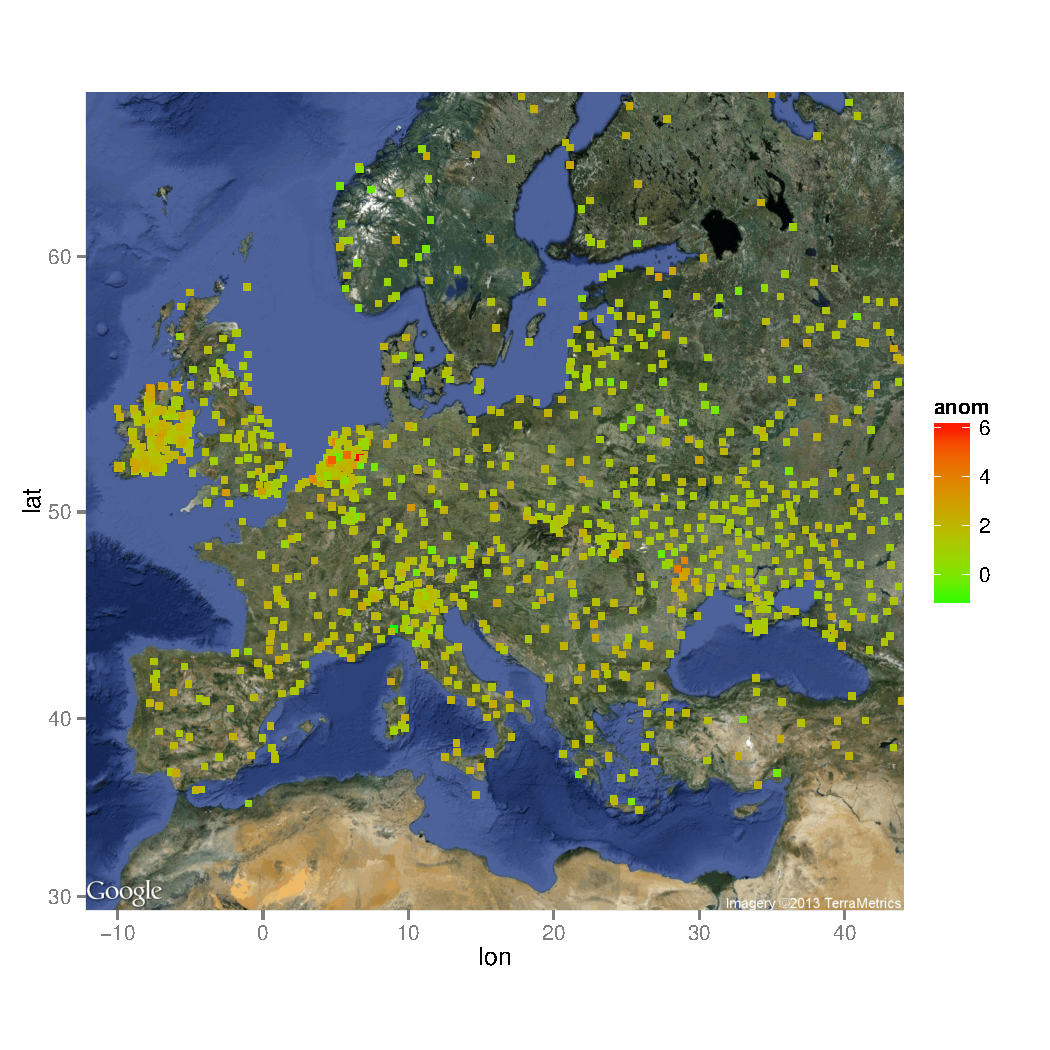
\includegraphics[width=5.5in]{figures/data.pdf}
\end{figure}

\subsection{The basic {\tt spacious} call}

The main call is

\begin{verbatim}
spacious(formula, data, S,
         cov = "exp", cov.inits, fixed = list(smoothness = 0.5),
         blocks = list(type = "cluster", nblocks = round(n/50)),
         nthreads=1, gpu=FALSE,
         B, neighbors)
\end{verbatim}

The response and mean trend are specified by {\tt formula}, which follows the usual {\tt response $\sim$ sum of predictors} notation.
The optional data frame {\tt data} can be used to specify the variables in {\tt formula}.
The fit with longitude, latitude, and elevation as predictors with default exponential covariance and blocking options is

\begin{verbatim}
> fit <- spacious(anom ~ lon + lat + elev, S=S, data=anom.2011)
> summary(fit)
Coefficients:
   Estimate Std Err P-value
b0  1.84658 2.5e-01 4.2e-13
b1  0.00034 2.6e-03 9.0e-01
b2 -0.00567 4.9e-03 2.5e-01
b3 -0.00001 3.4e-05 7.6e-01
Spatial parameters
             Estimate Std Err
Nugget          0.319  0.0084
Partial Sill    0.055  0.0129
Range           3.072  1.0475
\end{verbatim}

Figure \ref{f:converge} gives the convergence plot that results from {\tt plot(fit)}.
This plots the value of each spatial covariance parameter at each iteration of the optimization routine.
When the model fit converges, these trace plots will plateau for all covariance parameters.
Model convergence can be assessed with the variable {\tt fit\$convergence}.
When {\tt fit\$convergence} is {\tt FALSE}, this plot may help identify which parameter(s) are not converging.

\begin{figure}
	\caption{Convergence plot for the temperature data.}\label{f:converge}
	\centering
	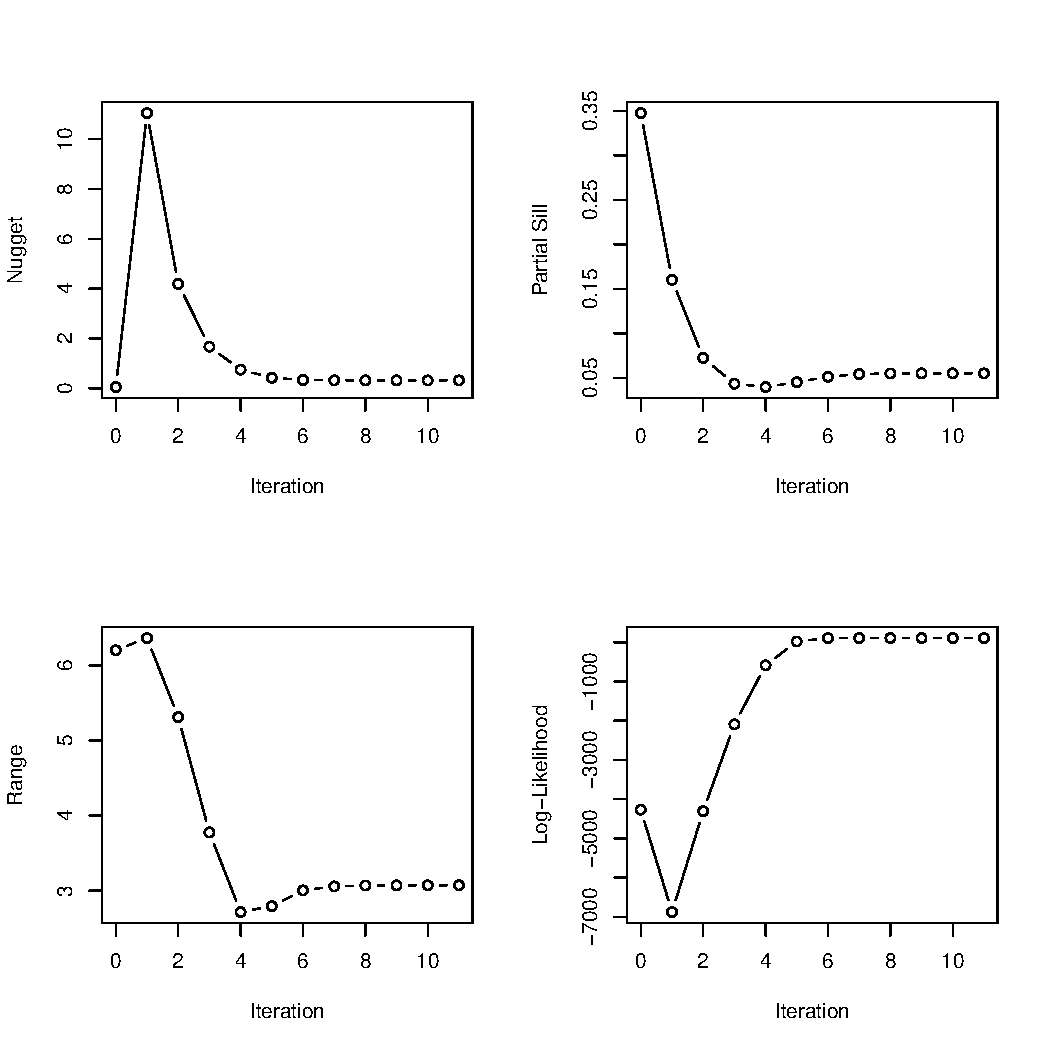
\includegraphics[width=3in]{figures/converge.pdf}
\end{figure}

\subsection{Specifying the spatial covariance function}
The default spatial covariance function is exponential covariance with the nugget, partial sill, and range to be estimated.
It is also possible to fix (rather than estimate) some of the parameters using the {\tt fixed} option, which is a list with three possible entries: {\tt nugget}, {\tt partial$\underline{\ }$sill}, and {\tt range}.
For example, {\tt fixed = list(nugget=0)} specifies a spatial covariance with no nugget ($\tau^2=0$).
Removing the nugget can lead to computational problems due to singular covariance matrices and should be used with caution.
Here is the fit with $\phi=5$,

\begin{verbatim}
> fit <- spacious(anom ~ lon + lat + elev, S=S, data=anom.2011,
                  fixed=list(range=5))
> summary(fit)
Coefficients:
   Estimate Std Err P-value
b0  1.8e+00 3.0e-01 1.9e-09
b1  4.9e-04 3.2e-03 8.8e-01
b2 -5.2e-03 5.8e-03 3.7e-01
b3 -1.4e-05 3.2e-05 6.7e-01
Spatial parameters
             Estimate Std Err
Nugget          0.325  0.0075
Partial Sill    0.053  0.0151
Range           5.000  0.0000
\end{verbatim}

{\tt Spacious} can also accommodate the $\Matern$ covariance using the {\tt cov="matern"} option.
In this case the smoothness parameter $\nu$ must be specified as fixed.
For example, the code below fits a $\Matern$ covariance with $\nu=1$,

\begin{verbatim}
> fit <- spacious(anom ~ lon + lat + elev, S=S, data=anom.2011,
                  cov="matern", fixed=list(smoothness=1))
> summary(fit)
Coefficients:
   Estimate Std Err P-value
b0  1.8e+00 2.4e-01 4.7e-14
b1  3.1e-04 2.5e-03 9.0e-01
b2 -5.6e-03 4.7e-03 2.3e-01
b3 -1.1e-05 3.3e-05 7.4e-01
Spatial parameters
             Estimate Std Err
Nugget          0.325  0.0074
Partial Sill    0.048  0.0117
Range           4.134  1.0901
Smoothness      1.000  0.0000
\end{verbatim}

Initial values for the spatial covariance parameters can be specified using the {\tt cov.inits} option, which is a list of the same form as {\tt fixed}.   The defaults are
\begin{verbatim}
cov.inits = list(nugget = 0.8*var(Y),
                 partial_sill = 0.2*var(Y),
                 range = quantile(dist(S),0.1))
\end{verbatim}
It is highly recommended to try several initial values to ensure they all lead to the same solution.

\subsection{Specifying the blocking structure}

Selecting the blocking structure that forms the block composite likelihood is a crucial step in applying {\tt spacious}.
Selecting one or two blocks gives the statistically optimal, but computationally inefficient, full likelihood.
Selecting a large number of blocks improves computational speed with a trade-off in statistically efficiency.
The blocking structure is determined by the {\tt blocks} argument, which is specified as a list with two elements: {\tt type} and {\tt nblocks}.
The {\tt type} argument can be either ``cluster'' or ``regular'', and {\tt nblocks} gives the number of blocks ($M$).
If {\tt type = "cluster"}, then the block groups are determined by k-means clustering of the observation locations, {\tt S}.
If {\tt type = "regular"}, then blocks are taken to be a regular $\sqrt{M}\times\sqrt{M}$ rectangular grid covering the range of {\tt S}.
Clearly, if {\tt type = "regular"}, then {\tt nblocks} should be a square number.
The default is cluster blocks with approximately $n/50$ blocks.

The following code fits the composite likelihood with $M=100$ blocks using both clustered and regular blocks:

\begin{verbatim}
> library(maps)
> fit_c <- spacious(anom ~ lon + lat + elev, S=S, data=anom.2011,
                    blocks=list(type="cluster", nblocks=100))
> fit_r <- spacious(anom ~ lon + lat + elev, S=S, data=anom.2011,
                    blocks=list(type="regular", nblocks=100))

> plot(S, cex=0.5, pch=19, axes=FALSE, main="Cluster blocks")
> map("world", add=TRUE, col=3)
> plot(fit_c$grid, add=TRUE)

> plot(S, cex=0.5, pch=19, axes=FALSE, main="Regular blocks")
> map("world", add=TRUE, col=3)
> plot(fit_r$grid, add=TRUE)
\end{verbatim}

The output {\tt B} gives the cluster label assigned to each observation, and is plotted in Figure~\ref{f:blocks}.
For these data, the regular blocks have many observations in two blocks in Ireland and the Netherlands, which slows computation.

\begin{figure}
	\caption{Blocking structures for the temperature data.}\label{f:blocks}
	\centering
	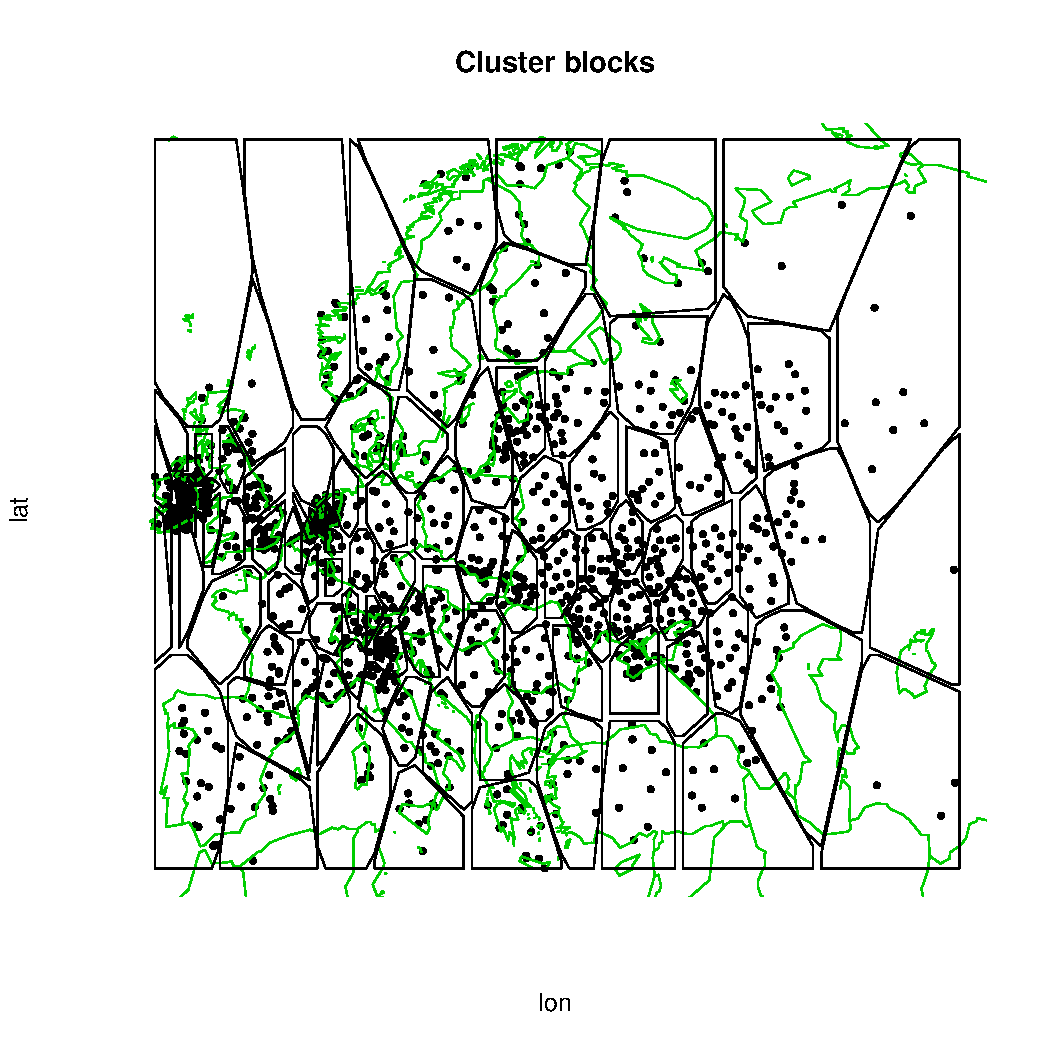
\includegraphics[width=3in]{figures/blocks_c.pdf}
	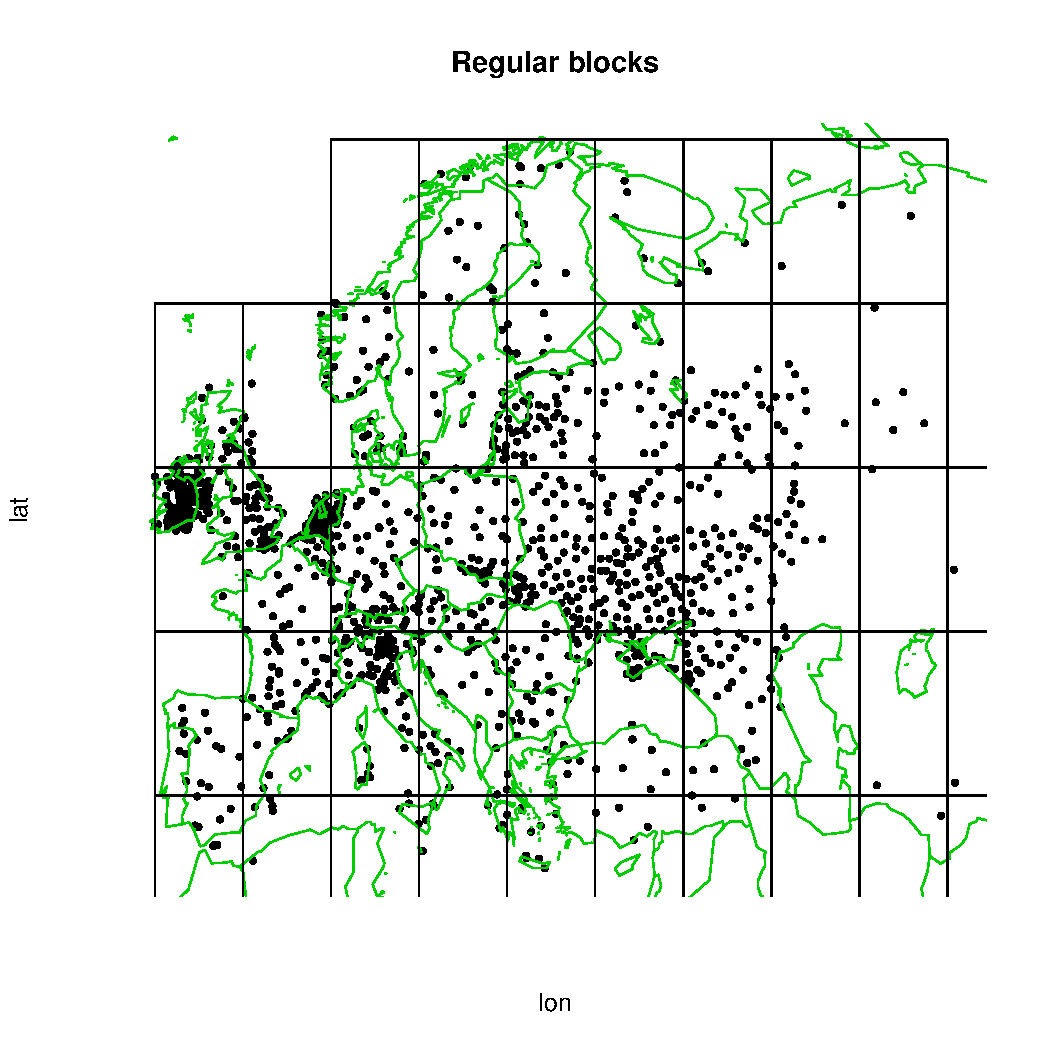
\includegraphics[width=3in]{figures/blocks_r.pdf}
\end{figure}

Alternatively, it is possible to specify the blocking structure directly using the {\tt B} and {\tt neighbors} arguments.
The input {\tt B} is a vector of $n$ block numbers (e.g., {\tt B[4] = 3} implies that the fourth observation is from block number 3), and {\tt neighbors} is an $M\times 2$ matrix specifying the adjacency structure of the blocks (e.g., if a row of {\tt neighbors} equals {\tt c(4,5)} then blocks 4 and 5 are neighbors).

\section{Spatial prediction}\label{s:predict}

Spatial prediction is carried out using the {\tt predict} function.
The required arguments are the {\tt spacious} fit, the prediction locations, {\tt newS}, and any covariates, {\tt newdata}.
The code below generates fitted values at locations {\tt Sp}, and plots the fitted values using ggmaps (Figure~\ref{f:pred}).

\begin{verbatim}
> fit  <- spacious(anom ~ lon + lat + elev, S=S, data=anom.2011)
> Sp   <- cbind(anom.pred.grid$lon, anom.pred.grid$lat)
> pred <- predict(fit, newdata=anom.pred.grid, newS=Sp)$y

> ggmap(euro) +
      geom_point(aes(lon, lat, color=pred), shape=15, size=1.25,
                 data=data.frame(anom.pred.grid, pred=pred)) +
      scale_colour_gradient(low = "green", high="red")
\end{verbatim}

\begin{figure}
	\caption{Spatial predictions for the temperature (Celcius) anomaly data.}\label{f:pred}
	\centering
	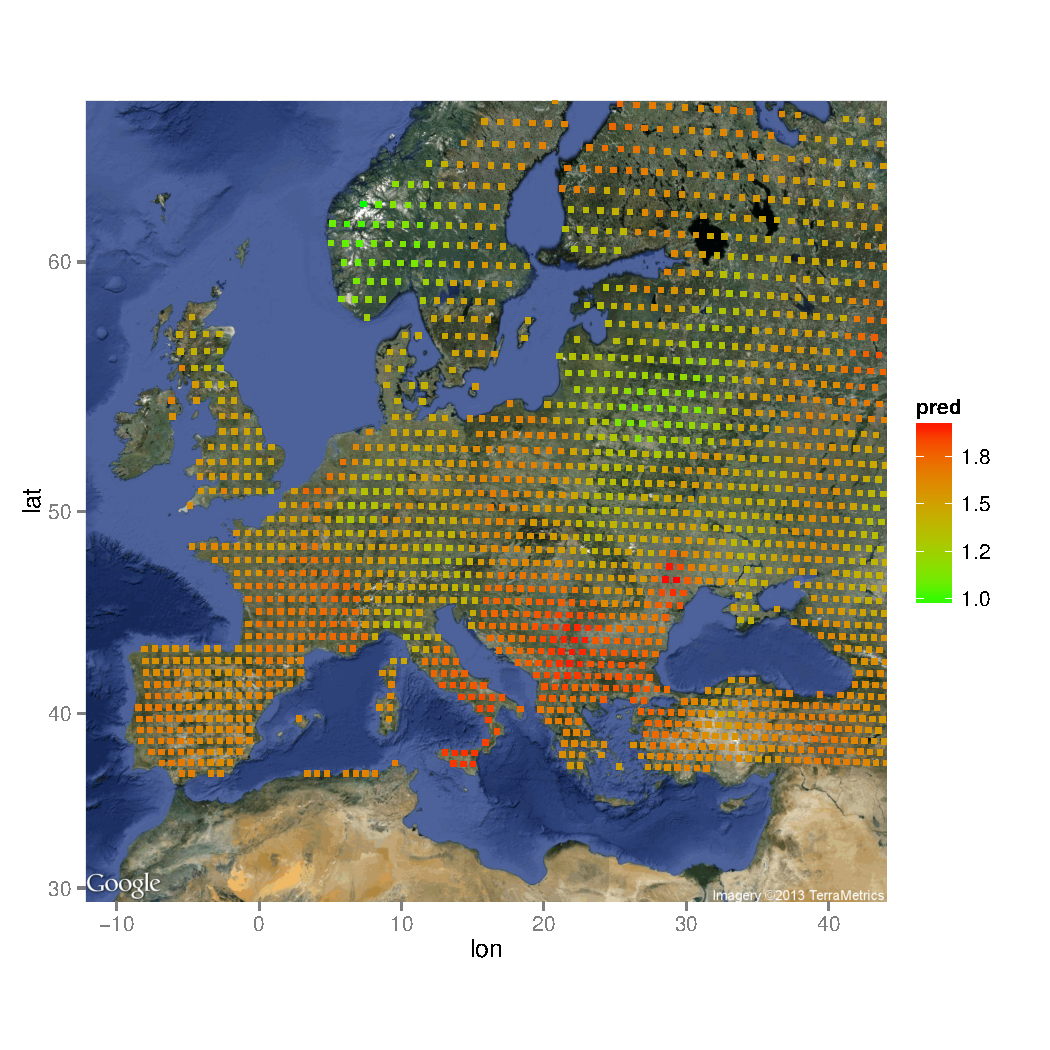
\includegraphics[width=6in]{figures/pred.pdf}
\end{figure}


By default, {\tt predict} uses block prediction \citep{Eidsvik:2013} with blocks specified by the {\tt spacious} object.
Alternatively, the {\tt opts} argument can be used to perform local prediction where only the closest $m$ locations to each prediction point are used for prediction (so that taking $m=n$ gives the usual Kriging predictions).
The code below uses the nearest $m=25$ observations for prediction, which gives similar results to the block predictions.

\begin{verbatim}
> pred.local <- predict(fit, newdata=anom.pred.grid, newS=Sp,
                        opts=list(type="local", num=25))$y
> pred[1:5]
[1] 1.663 1.651 1.616 1.610 1.614
> pred.local[1:5]
[1] 1.660 1.648 1.605 1.595 1.599
\end{verbatim}

Prediction intervals can also be obtained by adding the argument {\tt interval="prediction"} and optionally specifying confidence {\tt level} (default is 0.95).
For example, the 95\% prediction intervals for the first five prediction locations are

\begin{verbatim}
> predict(fit, newdata=anom.pred.grid[1:5,], newS=Sp[1:5,], interval="prediction")
      y     sd    lwr   upr
1 1.663 0.5953 0.4958 2.829
2 1.651 0.5942 0.4860 2.815
3 1.616 0.5975 0.4445 2.787
4 1.610 0.6000 0.4342 2.786
5 1.614 0.6077 0.4234 2.805
\end{verbatim}

\section{Estimation with parallel computing for large data sets}\label{s:parallel}

\section*{Acknowledgments}

\begin{singlespace}
	\bibliographystyle{asa.bst}
	\bibliography{spacious_manual}
\end{singlespace}

\end{document}

